\documentclass[journal,12pt,twocolumn]{IEEEtran}

\usepackage{setspace}
\usepackage{gensymb}
\singlespacing
\usepackage[cmex10]{amsmath}

\usepackage{amsthm}
\usepackage{amsmath,amssymb}
\usepackage{mathrsfs}
\usepackage{txfonts}
\usepackage{stfloats}
\usepackage{bm}
\usepackage{cite}
\usepackage{cases}
\usepackage{subfig}

\usepackage{longtable}
\usepackage{multirow}

\usepackage{enumitem}
\usepackage{mathtools}
\usepackage{steinmetz}
\usepackage{tikz}
\usepackage{circuitikz}
\usepackage{verbatim}
\usepackage{tfrupee}
\usepackage[breaklinks=true]{hyperref}
\usepackage{graphicx}
\usepackage{tkz-euclide}

\usetikzlibrary{calc,math}
\usepackage{listings}
    \usepackage{color}                                            %%
    \usepackage{array}                                            %%
    \usepackage{longtable}                                        %%
    \usepackage{calc}                                             %%
    \usepackage{multirow}                                         %%
    \usepackage{hhline}                                           %%
    \usepackage{ifthen}                                           %%
    \usepackage{lscape}     
\usepackage{multicol}
\usepackage{chngcntr}

\DeclareMathOperator*{\Res}{Res}

\renewcommand\thesection{\arabic{section}}
\renewcommand\thesubsection{\thesection.\arabic{subsection}}
\renewcommand\thesubsubsection{\thesubsection.\arabic{subsubsection}}

\renewcommand\thesectiondis{\arabic{section}}
\renewcommand\thesubsectiondis{\thesectiondis.\arabic{subsection}}
\renewcommand\thesubsubsectiondis{\thesubsectiondis.\arabic{subsubsection}}


\hyphenation{op-tical net-works semi-conduc-tor}
\def\inputGnumericTable{}                                 %%

\lstset{
%language=C,
frame=single, 
breaklines=true,
columns=fullflexible
}
\makeatletter
\setlength{\@fptop}{0pt}
\makeatother
\begin{document}

\newcommand{\BEQA}{\begin{eqnarray}}
\newcommand{\EEQA}{\end{eqnarray}}
\newcommand{\define}{\stackrel{\triangle}{=}}
\bibliographystyle{IEEEtran}
\raggedbottom
\setlength{\parindent}{0pt}
\providecommand{\mbf}{\mathbf}
\providecommand{\pr}[1]{\ensuremath{\Pr\left(#1\right)}}
\providecommand{\qfunc}[1]{\ensuremath{Q\left(#1\right)}}
\providecommand{\sbrak}[1]{\ensuremath{{}\left[#1\right]}}
\providecommand{\lsbrak}[1]{\ensuremath{{}\left[#1\right.}}
\providecommand{\rsbrak}[1]{\ensuremath{{}\left.#1\right]}}
\providecommand{\brak}[1]{\ensuremath{\left(#1\right)}}
\providecommand{\lbrak}[1]{\ensuremath{\left(#1\right.}}
\providecommand{\rbrak}[1]{\ensuremath{\left.#1\right)}}
\providecommand{\cbrak}[1]{\ensuremath{\left\{#1\right\}}}
\providecommand{\lcbrak}[1]{\ensuremath{\left\{#1\right.}}
\providecommand{\rcbrak}[1]{\ensuremath{\left.#1\right\}}}
\DeclarePairedDelimiter\ceil{\lceil}{\rceil}
\DeclarePairedDelimiter\floor{\lfloor}{\rfloor}
\theoremstyle{remark}
\newtheorem{rem}{Remark}
\newcommand{\sgn}{\mathop{\mathrm{sgn}}}
\providecommand{\abs}[1]{\vert#1\vert}
\providecommand{\res}[1]{\Res\displaylimits_{#1}} 
\providecommand{\norm}[1]{\lVert#1\rVert}
%\providecommand{\norm}[1]{\lVert#1\rVert}
\providecommand{\mtx}[1]{\mathbf{#1}}
\providecommand{\mean}[1]{E[ #1 ]}
\providecommand{\fourier}{\overset{\mathcal{F}}{ \rightleftharpoons}}
%\providecommand{\hilbert}{\overset{\mathcal{H}}{ \rightleftharpoons}}
\providecommand{\system}{\overset{\mathcal{H}}{ \longleftrightarrow}}
	%\newcommand{\solution}[2]{\textbf{Solution:}{#1}}
\newcommand{\solution}{\noindent \textbf{Solution: }}
\newcommand{\cosec}{\,\text{cosec}\,}
\providecommand{\dec}[2]{\ensuremath{\overset{#1}{\underset{#2}{\gtrless}}}}
\newcommand{\myvec}[1]{\ensuremath{\begin{pmatrix}#1\end{pmatrix}}}
\newcommand{\mydet}[1]{\ensuremath{\begin{vmatrix}#1\end{vmatrix}}}
\numberwithin{equation}{subsection}
\makeatletter
\@addtoreset{figure}{problem}
\makeatother
\let\StandardTheFigure\thefigure
\let\vec\mathbf
\renewcommand{\thefigure}{\theproblem}
\def\putbox#1#2#3{\makebox[0in][l]{\makebox[#1][l]{}\raisebox{\baselineskip}[0in][0in]{\raisebox{#2}[0in][0in]{#3}}}}
     \def\rightbox#1{\makebox[0in][r]{#1}}
     \def\centbox#1{\makebox[0in]{#1}}
     \def\topbox#1{\raisebox{-\baselineskip}[0in][0in]{#1}}
     \def\midbox#1{\raisebox{-0.5\baselineskip}[0in][0in]{#1}}
\vspace{3cm}
\title{Assignment 8}
\author{Chirag Mehta - AI20BTECH11006}
\maketitle
\newpage
\bigskip
\renewcommand{\thefigure}{\theenumi}
\renewcommand{\thetable}{\theenumi}
Download all python codes from 
\begin{lstlisting}
https://github.com/cmapsi/AI1103-Probability-and-random-variables/tree/main/Assignment-8/codes
\end{lstlisting}
and latex-tikz codes from 
\begin{lstlisting}
https://github.com/cmapsi/AI1103-Probability-and-random-variables/blob/main/Assignment-8/main.tex
\end{lstlisting}
\section{Problem}
(CSIR UGC NET EXAM (Dec 2015), Q.106) Let $X_1,X_2,...,X_n$ be independent and identically distributed, each having a uniform distribution on $(0,1)$. Let $S_n=\sum_{i=1}^{n}X_i$ for $n\ge 1$. Then, which of the following statements are true? 
\begin{enumerate}[label=\Alph*)]
\item $\frac{S_n}{n \log{n}}\to 0 \text{ as } n \to \infty$ with probability 1.
\item $\pr{\brak{S_n>\frac{2n}{3}}\text{occurs for infinitely many n}}=1$
\item $\frac{S_n}{\log{n}}\to 0\text{ as } n \to \infty$ with probability 1.
\item $\pr{\brak{S_n>\frac{n}{3}}\text{occurs for infinitely many n}}=1$
\end{enumerate}
\section{solution}

\begin{table}[htp]
\centering
    \resizebox{\columnwidth}{25mm}{
\begin{tabular}{ |c|c|c|} 
\hline
\textbf{Symbol} & \textbf{expression/definition} \\
\hline
$S_n$ & $\displaystyle \sum_{i=1}^{n}X_i$  \\
\hline
$\mu_n$ & $\displaystyle \frac{1}{n} \sum_{i=1}^{n}X_i$  \\
\hline
& Independent continuous random\\$X$&variable identical to $X_1,X_2,...,X_n$ \\
\hline
\end{tabular}}
\caption{Variables and their definitions}
\label{table1}
\end{table}

Given
\begin{align}
\displaystyle S_n=\sum_{i=1}^{n}X_i , n\ge 1
\end{align}
Dividing by $n$ on both sides
\begin{align}
\dfrac{S_n}{n}=\displaystyle\frac{1}{n} \sum_{i=1}^{n}X_i=\mu_n
\end{align}
It can be said that $X_1,X_2,...,X_n$ are the trials of $X$. By definition
\begin{align}
E\sbrak{X}&=\displaystyle \lim_{n\to \infty} \frac{\sum_{i=1}^{n}X_i}{n}=\lim_{n\to \infty} \frac{S_n}{n}\\
&\lim_{n\to \infty} \frac{S_n}{n}=E\sbrak{X}=\frac{1}{2} \label{eq:mu_value} \\
\therefore&\lim_{n\to \infty} \frac{S_n}{n\log{n}}=0
\end{align}
It is easy to observe from \eqref{eq:mu_value} that option C is false.\\
Using weak law, \eqref{eq:mu_value}, and table \eqref{table1}
\begin{align}
\lim_{n\to\infty} \pr{\abs{\mu_n-E\sbrak{x}}>\epsilon}=0, \forall \epsilon >0 \label{eq:weak_law}
\end{align}
\begin{align}
\therefore \pr{\brak{S_n>\frac{n}{3}}\text{occurs for infinitely many n}}=1
\end{align}
It can be easily implied from \eqref{eq:weak_law} that option B is false.

\begin{figure}[ht]
\centering
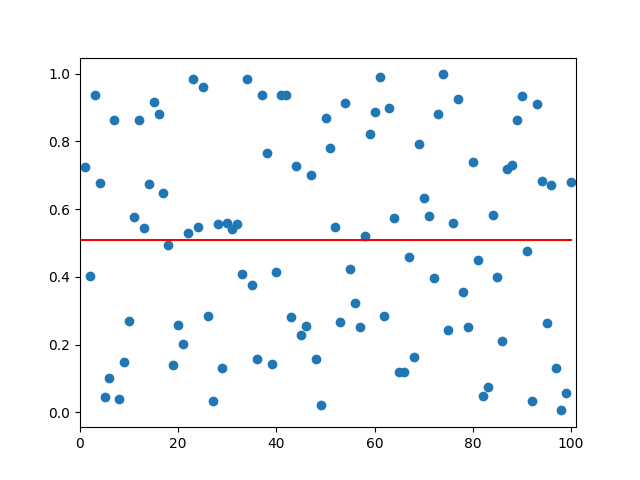
\includegraphics[width=\linewidth]{figure/fig}
\caption{Mean simulation with n=100}
\label{plot}
\end{figure}

\end{document}
